\documentclass[12pt,UTF8,a4paper]{ctexart}
\usepackage[margin=2.5cm]{geometry}
\usepackage{graphicx}
\graphicspath{{figures/}}
\usepackage{booktabs}
\usepackage{amsmath}
\usepackage{caption}
\usepackage{hyperref}
\captionsetup{font=small}
\setlength{\parskip}{0.5em}

\title{\textbf{自主空战导引与机炮攻击}\\[0.5em]
\large SimplePlanes 2 飞行控制学习项目·SC-2 验证试验报告}
\author{}
\date{2026 年 9 月 22 日}

\begin{document}
\maketitle
\thispagestyle{empty}

\begin{abstract}
本报告记录 SC-2 课题（高性能验证机 TESTfighter 的自主空中截获与机炮攻击）的导引控制律设计与试飞验证结果。经多轮迭代定版的三通道控制律（滚转全空域小角度跟踪、俯仰绝对姿态目标配地面联锁、能量自主管理）在实飞中完成从 22 km 外截获、连续跟踪、终端穿越至机炮击落敌机的完整杀伤链，并建立了以机载多源遥测与几何残差配对为基础的全链路离线重建评估方法。试验判定：导引律主链路验收通过；命中提前量与不对称挂载静差列为遗留项。下一课题为 SC-3 自动着陆。
\end{abstract}

\section{试验背景与平台}
被试平台为自主设计的鸭式喷气验证机 TESTfighter（双军用涡扇，推重比 1.79，主翼面积 21.8 m$^2$）：实测最大平飞速度超过 340 m/s，持续滚转率 100--190$^\circ$/s，俯仰姿态权限 35--55$^\circ$/s 不饱和，过载 p95 为 8.8 g（240 m/s）——三项指标均为上一平台 TESTaircraft 的 3--8 倍，控制律需在新权限域内重新设计而非移植。

控制架构沿用已封版的分层方案：快回路（舵面内环、导引律）由机载表达式引擎（Funky Trees，每物理拍位置式求值）实现；慢回路（能量管理、模式守护、遥测）由 MFD Lua 脚本以真时间步长实现。目标信息经表达式侧只读变量获取：目标选定标志（TargetSelected）、目标方位（TargetHeading）、目标视线仰角（TargetElevation）与斜距（TargetDistance）。

\section{评估方法与观测体系}
本课题建立了完整的量化评估链路，其要点如下：
\begin{itemize}
\item \textbf{多流分离}：同场景内多架带记录设备的航空器共用一份日志，逐流附加实例身份列，按时间回退切分架次，杜绝混流统计；
\item \textbf{位姿与目标流}：每机按 10 Hz 记录世界坐标（POS 流）与跟踪目标距离（SEEK 流）；
\item \textbf{几何配对}：以两机间距与报告斜距之残差 $|d_{12}-D_{\mathrm{rep}}|\approx 0$ 唯一确定本机所追目标，残差达百米级即判配对失败，防止张冠李戴；
\item \textbf{离线 1:1 重建}：由双方轨迹复算方位误差 $\varepsilon$、视线高低角、视线转率 $\dot\lambda$、坡度指令与实际滚转角的跟随误差等全部制导量，使"指令—执行—收敛"三环均可分别裁决。
\end{itemize}
该方法在多轮改型中每次都成功定位了问题环节（阻尼配比、映射定义域、目标数据失效等），是本轮工程迭代的主要依据。

\section{导引控制律设计（定版）}
\subsection{符号与几何}
$\varepsilon=\mathrm{wrap}(H_t-H)$ 为目标方位与本机航向的最短角差（右为正）；视线转率 $\dot\lambda=\mathrm{rate}(\varepsilon)+\mathrm{clamp}(\mathrm{rate}(H),-30,30)$（补回本机偏航，得惯性系真实转率）；准星高低角 $V_{\!ps}=\theta_{\mathrm{elev}}+\alpha-\theta$（目标视线仰角、迎角、俯仰角）。

\subsection{滚转通道}
定版律为全空域统一的小角度跟踪形式：
\[
\varphi_c=\mathrm{clamp}\!\bigl(6\,\varepsilon+4\,\dot\lambda,\ \pm85^\circ\bigr),
\qquad
\delta_a=\mathrm{clamp}\!\bigl(R+0.10(\varphi-\varphi_c)+0.004\,p,\ \pm1\bigr).
\]
方位偏差 15$^\circ$ 即请求满坡度，收敛速度优先；$\dot\lambda$ 项提供前摄与阻尼。内环阻尼系数经试飞标定：0.014 在快速压坡（$p\approx150^\circ$/s）时产生 2.1 的反向舵量、将 85$^\circ$ 指令压至实际 40$^\circ$，降至 0.004 后指令—执行偏差消除。设计过程中亦曾采用纯比例导引（$\varphi_c=\arctan(NV\dot\lambda/g)$）与反正切几何式，前者对大方位差、低转率工况（目标居侧方）响应不足，后者在 $|\varepsilon|>90^\circ$ 出现主值折叠使掉头指令趋零，均被试验驳回后回退，记录于 \S5。

\subsection{俯仰通道}
绝对姿态目标律：
\[
\theta_d=\theta_{\mathrm{elev}}+\alpha-\eta\qquad(\text{AGL}<400\ \mathrm{m}\ \text{时取下界}\ 5^\circ),
\]
\[
\delta_e=\mathrm{clamp}\!\bigl(T+\mathrm{PID}(\theta_d-10s_\theta,\ \theta,\ -0.35,\ 0,\ -0.008),\ \pm1\bigr),
\]
挂点角 $\eta$：常态 1$^\circ$（目标悬于准星上方，即"拉杆穿越"射击几何）；捕获态 $\eta=0$。捕获判据 TRV $=|\varepsilon|<4^\circ$（全距离，不设近距门）。姿态误差 3$^\circ$ 即满舵，俯仰速率顶至机体物理上限（35--55$^\circ$/s）；$-10s_\theta$ 项保留驾驶杆姿态越权通道。AGL 联锁为安全件：追低目标曾致受控飞行撞地（CFIT）工况，律在 400 m 以下强制退出俯冲。

\subsection{火控与系统守护}
机炮指令 $\delta_{\mathrm{gun}}=\mathrm{FireGuns}\ \lor\ (\mathrm{TRV}\land D<2\,\mathrm{km}\land|V_{\!ps}|<0.5^\circ)$，即穿越准星瞬间自动短点射。能量管理：武器通电且离地后油门恒推进满舵，仅 250 m/s 以上压回 0.5 削峰——此前"机动速度带"方案因切断油门与解除门耦合形成能量单向流失，已废止。目标数据失效守护：斜距 5 s 冻结判为幽灵锁定，自动断开目标模式，导引律即时释放交还操纵。

\section{试飞结果}
\begin{itemize}
\item \textbf{完整杀伤链}：对活动靶机自 3.6 km 截获，28 s 内完成对准—跟踪—穿越—射击，\textbf{击落目标}（项目首例机炮毁伤）；
\item \textbf{截获能力}：22 km、初始方位差 155$^\circ$ 条件下持续跟踪 260 s、最近逼近 7 m，全程滚转指令—实际跟随误差中位数 0.7$^\circ$；
\item \textbf{收敛速度}：定版律下 40 s 由 8.9 km 收至 730 m（平均闭率 $\approx$200 m/s）；准星穿越 15 次、捕获态累计 12.1 s；
\item \textbf{能量守护}：修复油门泄漏后未再出现速度塌陷；俯仰通道自地面联锁入列后零 CFIT、零短周期振荡；
\item \textbf{高度保持}：AP 俯仰振荡定位为表达式重写改变轴—舵面链路增益（0.5$\to$3.5）而 Lua 内环未折算，按有效舵量折算后消除。
\end{itemize}
图 \ref{fig:axial} 给出典型接敌段全链路重建（指令、实际姿态、距离、过载共五通道）。

\begin{figure}[htbp]\centering
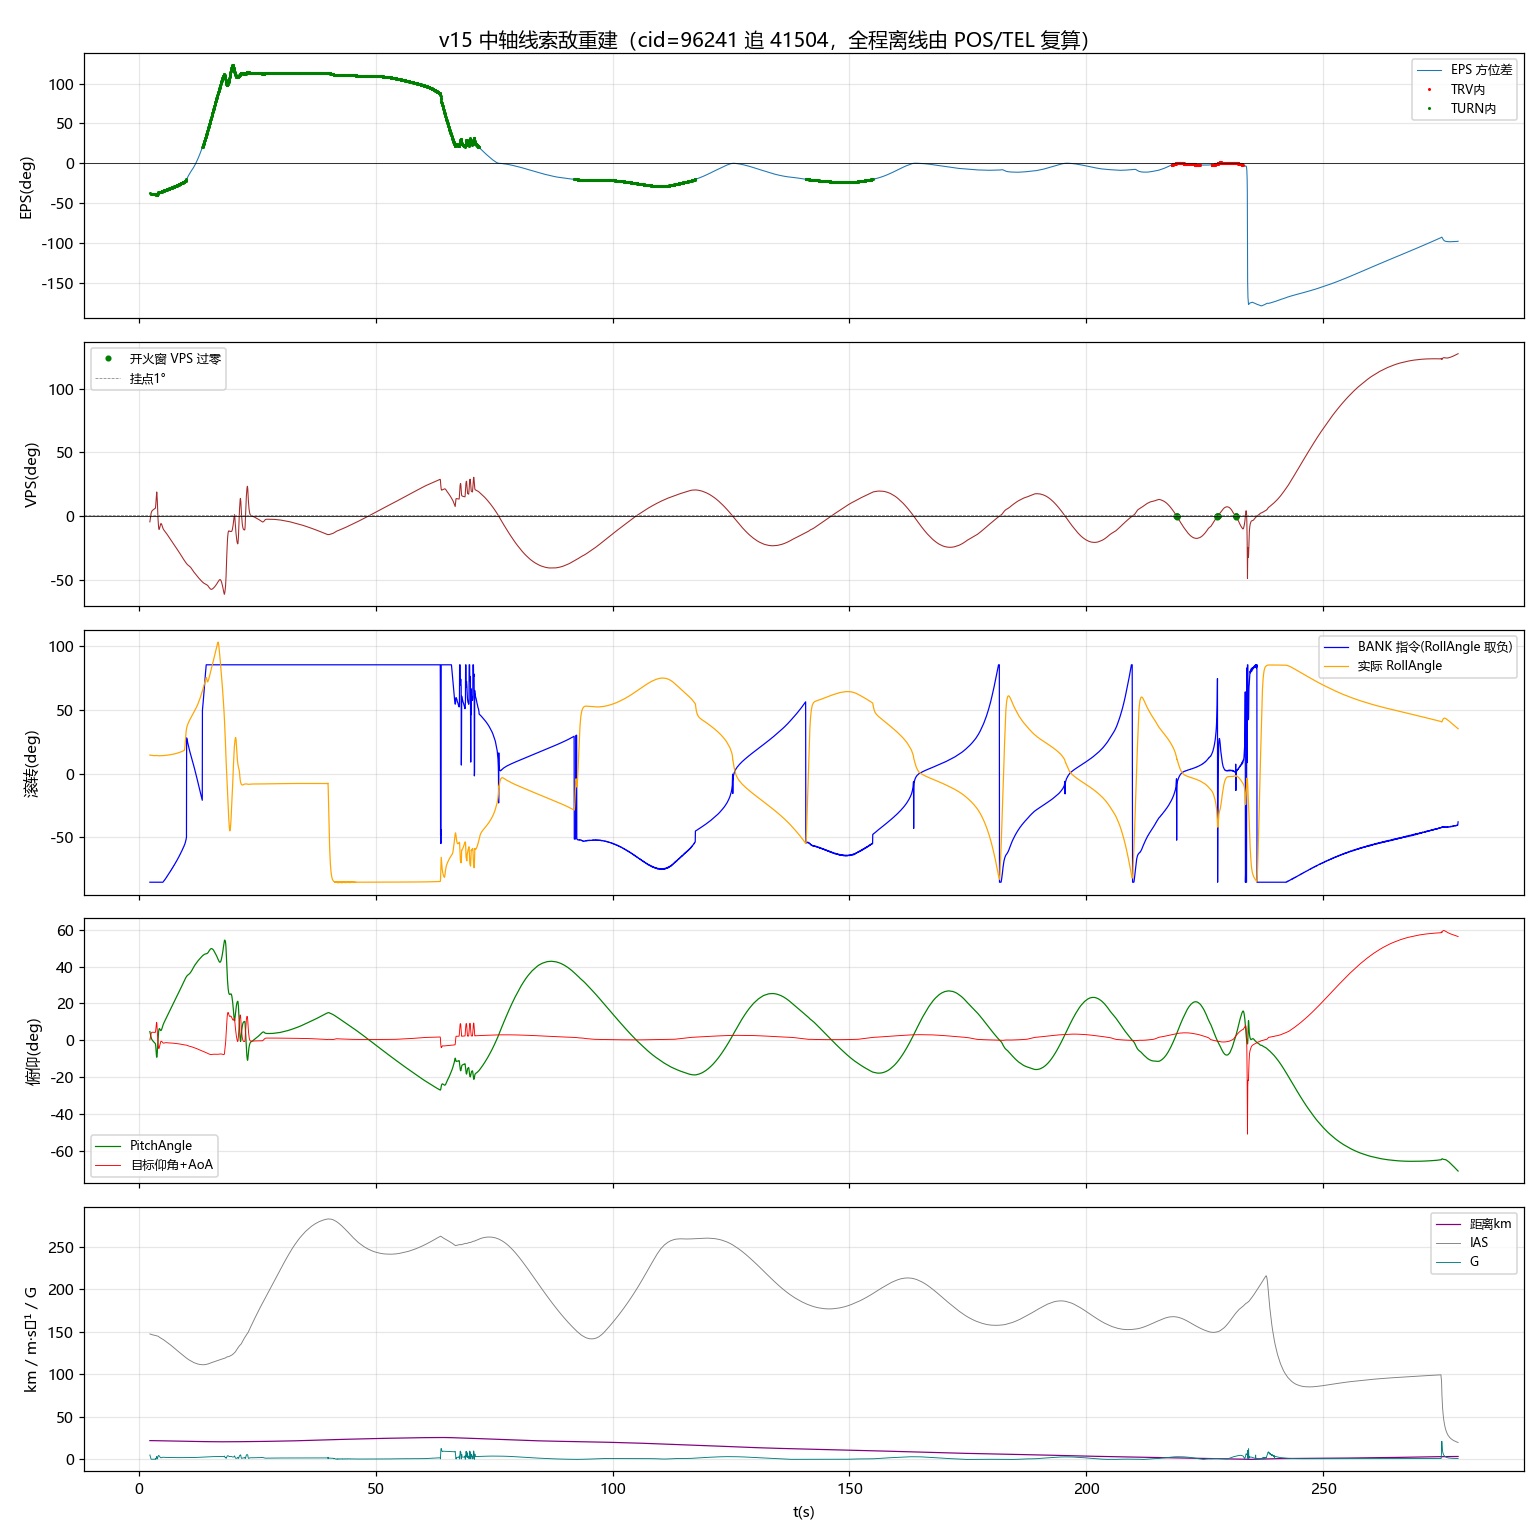
\includegraphics[width=0.98\textwidth]{v15-axial-report.png}
\caption{接敌段离线重建：方位误差、准星高低角（含穿越与射击窗标记）、坡度指令与实际、俯仰、距离/速度/过载}
\label{fig:axial}
\end{figure}

\section{设计评述}
本课题的迭代成本主要消耗在四类方法性问题上，均有量化证据，列为后续设计守则：
\begin{enumerate}
\item \textbf{映射的定义域检验}：任何"角度$\to$坡度"类映射须检验全域（含 $|\varepsilon|\to180^\circ$、分母$\to0$ 邻域）的增益有界性与连续性——反正切折叠与反正切小分母悬崖各造成一类失效；
\item \textbf{量纲一致性}：转弯率由 $g\tan\varphi/V$ 决定，坡度指令应经转率需求折算，误差角的线性增益定标须换算为等效转率再与机体权限对表；
\item \textbf{跨通道增益折算}：任一通道的律重写会改变"轴指令—舵面"链路增益，其余通道的整定参数须联动审计（AP 俯仰振荡案）；
\item \textbf{指令保持与释放纪律}：一切覆写型执行通道必须定义死区外的释放路径，否则形成操纵悬挂（油门 0.5 卡死案）。
\end{enumerate}

\section{结论与展望}
SC-2 主链路（截获—跟踪—穿越—射击—命中）验收通过，导引律进入冻结状态；遗留两项：横向机动目标的命中提前量（拟按比例导引前置角项引入，待批准）、不对称挂载下的滚转静差（P 型内环结构性静差，裁定以配平操纵吸收，不加机载积分）。下一课题 SC-3：自动着陆（进近—下滑—平飘—触地—减速滑跑），平台侧通道已具备起落架、襟翼、刹车与无线电高度。

\end{document}
